\chapter{2018}
\section*{一、选择题(本大题共 15 小题,每小题 2 分,共 30 分)}

1. 下面程序段的时间复杂度是(   )。
\begin{lstlisting}[language=C, basicstyle=\ttfamily]
i = 1;
while(i <= n)
    i = i*3;
\end{lstlisting}

A.O(n) B. \(O\left( {{nlog}\left( n\right) }\right)\) C. \(\mathrm{O}\left( {\log \left( \mathrm{n}\right) }\right)\) D. \(O\left( {\log }_{3}^{n}\right)\)

2. 在 \(\mathrm{n}\) 个元素的顺序表中插入或删除一个元素,需要平均移动表中(   )个元素。

A. (n) B. \(\left( {\mathrm{n}/2}\right)\) C. \(\left( {\mathrm{n}}^{2}\right)\) D. (1)

3. 设循环队列中数组的下标范围是 \(0,\ldots ,\mathrm{m} - 1\) ,其头指针 front 指向队首元素, rear 指向队尾元素,则队列的长度为(   )。

A. (rear-front +1)\% (m +1) B. (rear-front \(+ \mathrm{m} + 1\) ) \(\% \mathrm{\;m}\)
C. rear-front D. rear-front +1

4. 设计一个十进制转换为八进制的算法,采用(   )数据结构最佳。

A. 栈 B. 队列

C. 顺序结构线性表 D. 链式结构线性表

5. 若某个栈的输入序列为 \(1,2,3,\ldots ,\mathrm{n}\) ,输出序列的第一个元素为 \(\mathrm{n}\) ,则第 \(\mathrm{i}\) 个输出元素为(   )。

A. i B. n-i C. n-i+1 D. 哪个元素无所谓

6. 六个元素按6,5,4,3,2,1的顺序进栈,下列哪个出栈序列是错误的 (   )。

A. 5 4 3 6 1 2 B. 4 5 3 1 2 6

C. 3 4 6 5 2 1 D. 2 3 4 1 5 6

7. 某二叉树的先序序列和后序序列正好相反,则该二叉树一定是(   )二叉树。

A. 空或只有一个结点 B. 高度等于其结点数

C. 任一结点无左孩子 D. 任一结点无右孩子

8. 高度为 \(\mathrm{k}\) 的完全二叉树至少有(   )个结点 ( 空树高度为 0 )。

A. \({2}^{\mathrm{k} - 1}\) B. \({2}^{\mathrm{k}}\)

C. \({2}^{\mathrm{k}} - 1\) D. \(\mathrm{k}\)

9. 设高度为 \(\mathrm{h}\) 的二叉树上只有度为 0 和度为 2 的结点,则此二叉树中至多有 (   )个结点。

A. \({2}^{\mathrm{h}} - 1\) B. \({2}^{h - 1}\) C. \({2}^{\mathrm{h}} + 1\) D. \({2}^{h + 1} - 1\)

10. 数组 A 中,每个元素的长度为 3 个字节,行下标 i 从 1 到 8 ,列下标 j 从 1 到 10 ,从首地址 SA 开始连续存放在存储器内,该数组按行优先存放时,元素 \(\mathrm{A}\left\lbrack  8\right\rbrack  \left\lbrack  5\right\rbrack\) 的起始地址为(   )。

A. SA+141 B. SA+222

C. SA+144 D. SA+225

11. 任何一个无向连通图的最小生成树(   )。

A. 有一棵或多棵 B. 一定只有一棵

C．一定有多棵 D. 可能不存在

12. 对于一个具有 \(\mathrm{n}\) 个顶点和 \(\mathrm{e}\) 条边的无向图,若采用邻接表表示,则表头向量的大小为 \(\mathrm{n}\) ；所有邻接表中的结点总数是(   )。

A. \(\mathrm{e}/2\) B.e C. 2e D.n+e

13. 设结点 \(\mathrm{x}\) 和结点 \(\mathrm{y}\) 是二叉树 \(\mathrm{T}\) 中的任意两个结点,若在先序序列中 \(\mathrm{x}\) 在 \(\mathrm{y}\) 之前,而在后序序列中 \(\mathrm{x}\) 在 \(\mathrm{y}\) 之后,则 \(\mathrm{x}\) 和 \(\mathrm{y}\) 的关系是 (   )

A. \(\mathrm{x}\) 是 \(\mathrm{y}\) 的左兄弟 B. \(\mathrm{x}\) 是 \(\mathrm{y}\) 的右兄弟
C. \(\mathrm{x}\) 是 \(\mathrm{y}\) 的祖先 D. \(\mathrm{x}\) 是 \(\mathrm{y}\) 的后代

14. 关于下面的图形,哪个说法正确(   )。

\begin{center}
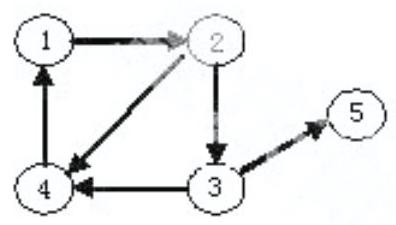
\includegraphics[width=0.3\textwidth]{images/2018/choice_14.jpg}
\end{center}
\hspace*{3em} 

A. 路径 \(< 1,2 > , < 2,4 > , < 4,1 >\) 是一条回路；

B. 顶点 2 的入度为 2 ；

C. 顶点 4 的出度为 2 ；

D. 以上皆非。

15. 下列序列中,(   )是执行第一趟快速排序后得到的序列(排序的关键字类型是字符串)。

A. \(\left\lbrack  {\mathrm{{da}},\mathrm{{ax}},\mathrm{{eb}},\mathrm{{de}},\mathrm{{bb}}}\right\rbrack\) ff \(\left\lbrack  {\mathrm{{ha}},\mathrm{{gc}}}\right\rbrack\) B. \(\left\lbrack  {{cd},{eb},{ax},{da}}\right\rbrack\) ff \(\left\lbrack  {{ha},{gc},{bb}}\right\rbrack\)

C. \(\left\lbrack  {\mathrm{{gc}},\mathrm{{ax}},\mathrm{{eb}},\mathrm{{cd}},\mathrm{{bb}}}\right\rbrack\) ff \(\left\lbrack  {\mathrm{{da}},\mathrm{{ha}}}\right\rbrack\) D. \(\left\lbrack  {{ax},{bb},{cd},{da}}\right\rbrack\) ff \(\left\lbrack  {{eb},{gc},{ha}}\right\rbrack\)

\section*{二、填空题(本大题共 10 小题,每小题 3 分,共 30 分)}

1. 采用顺序查找方法查找长度为 \(\mathrm{n}\) 的线性表时,在等概率情况下查找成功的平均查找长度为\_\_\_\_\_。

2. 已知数据表 A 中每个元素距其最终位置不远,则采用\_\_\_\_\_排序算法最节省时间。

3. 图 G 是一个非连通图,共有 28 条边,则该图至少有\_\_\_\_\_个顶点。

4. 设一循环队列 \(Q\) 中, rear 指针指向队尾元素的下一个位置, front 指针指向队首元素,则判断队列中元素为空的条件是\_\_\_\_\_。

5. 在大根堆中,关键字最小的元素可能存放在堆的任一\_\_\_\_\_结点上。

6. 某后缀表达式为 abcd-*+ef/-,令 a=2, b=3, c=4, d=5, e=6, f=2,则该表达

式的值等于\_\_\_\_\_。

7. 有 \(\mathrm{n}\) 个顶点的连通图用邻接矩阵表示时,该矩阵至少有\_\_\_\_\_个非零元素。

8. 高度(空树高度为 0)为 5 的 AVL 树,其结点数最少是\_\_\_\_\_。

9. 广义表((a),((b), c),(((d))))的长度是\_\_\_\_\_,深度是\_\_\_\_\_。

10. 在有 n 个结点的二叉链表中,空链域的个数为\_\_\_\_\_。

\section*{三、问答题(本大题共 6 小题,每小题 10 分,共 60 分)}

1. 已知二叉树的先序序列和中序序列分别为 ABDGCEFH 和 DGBAECHF:

(1) 画出该二叉树；

(2)写出此二叉树的后序序列；

(3)画出与此二叉树对应的森林。
\vspace{15em}

2. 图 G 各顶点的连接关系及相应权值如下图所示:

(1)画出图的邻接矩阵存储图示；

(2)从顶点 1 开始对图进行广度优先遍历,写出遍历结果；

(3)使用 Kruskal 算法求该图的最小生成树,给出形成过程。

\begin{center}
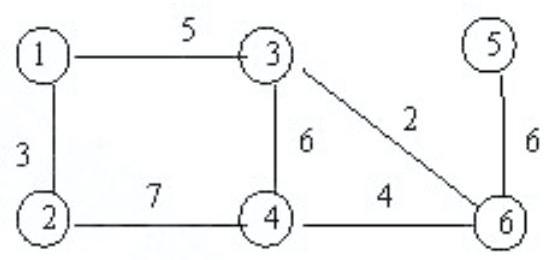
\includegraphics[width=0.4\textwidth]{images/2018/ask_2.jpg}
\end{center}
\hspace*{3em} 
\vspace{15em}

\newpage
3. 设散列表的长度为 8 ,散列函数 \(\mathrm{H}\left( \mathrm{k}\right)  = \mathrm{k}{\;\operatorname{mod}\;7}\) ,初始记录关键字序列为 (25,31,8,27,13,68),要求:

(1)分别给出用线性探测法和链地址法作为解决冲突方法的过程；

(2)计算(1)中两种解决冲突方法的平均查找长度。
\vspace{15em}

4. 已知一个图的顶点集 \(\mathrm{V}\) 和边集 \(\mathrm{E}\) 分别为:

\(\mathrm{V} = \{ 1,2,3,4,5,6,7\}\) ;

\(E = \{  < 2,1 > , < 3,2 > , < 3,6 > , < 4,3 > , < 4,5 > , < 4,6 > , < 5,1 > , < 5,7 > , < 6,1 > , < 6,2 > , < 6,5 > \} ;\)

若存储它采用邻接表, 并且每个顶点邻接表中的边结点都是按照终点序号从小到大的次序链接的,

(1)画出该图的邻接表存储图示；

(2)按拓朴排序算法进行排序,试给出得到的拓扑排序的序列。
\vspace{15em}

\newpage
5. 假设一个线性链表的类名为 linkedList, 链表结点的类名为 ListNode, 它包含两个数据成员 data 和 link。data 存储该结点的数据, link 是链接指针。下面给定一段递归打印一个链表中所有结点中数据的算法:

void PrintList (ListNode *L) \{

\hspace*{1em} if (L != NULL) \{

\hspace*{3em} printf("\%d ", L->data);

\hspace*{3em} PrintList (L->link);

\hspace*{1em} \}

\}

试问此程序在什么情况下不实用? 给出具体修改后的可实用的程序？
\vspace{15em}

6. 对于如下图所示的 AOE 网络,计算各活动弧的 \(e\left( {a}_{i}\right)\) (活动 \({a}_{i}\) 的最早开始时间)和 \(1\left( {a}_{j}\right)\) (活动 \({a}_{j}\) 的最迟开始时间)函数值、各事件(顶点)的 \({ve}\left( {v}_{i}\right)\) (事件 \({v}_{i}\) 的最早发生时间)和 \({vl}\left( {v}_{j}\right)\) (事件 \({v}_{j}\) 的最迟发生时间)函数值; 列出各条关键路径。

\begin{center}
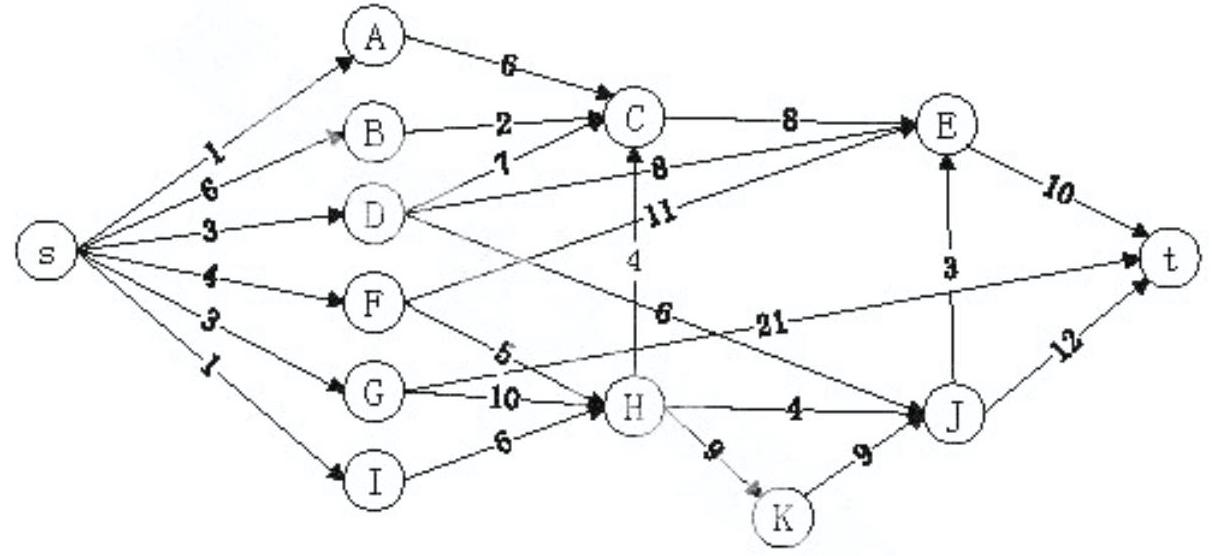
\includegraphics[width=1.0\textwidth]{images/2018/ask_6.jpg}
\end{center}
\hspace*{3em} 
\vspace{15em}

\section*{四、问答题(本大题共 2 小题,每小题 15 分,共 30 分)}

1. 现有关键字序列 \(\{ {45},{24},{37},{53},{12},{93},{47},{60}\}\) ,按以下要求完成:

(1)根据给定的关键字序列构造一棵二叉查找(排序)树,以二叉链表形式存储, 进行中序遍历可以得到从小到大排列的有序序列, 请写出构造过程 (不要求算法)。

(2)在(1)的基础上,请编写一个函数(int LeafCount(Binary\_tree BT),

求此二叉树的叶子结点个数。

有关的数据结构已描述如下:
\begin{lstlisting}[language=C, basicstyle=\ttfamily]
typedef struct { //二叉树结点
    int data;
    Binary_node *left;
    Binary_node *right;
} Binary_node, *Binary_tree;

int LeafCount(Binary_tree bt); //计算树bt的叶结点的个数
\end{lstlisting}
\vspace{45em}

2. 下面给出一个排序算法,其中 \(\mathrm{n}\) 是数据类型为 Type 的数组 \(\mathrm{A}\left\lbrack  \right\rbrack\) 中元素总数。

\begin{lstlisting}[language=C, basicstyle=\ttfamily]
void unknown(Type a[], int n)
{
    int d = 1;
    int j;
    while (d < n / 3)
        d = 3 * d + 1;
    while (d > 0)
    {
        for (int i = d; i < n; i++)
        {
            Type temp = a[i];
            j = i;
            while (j >= d && a[j - d] > temp)
            {
                a[j] = a[j - d];
                j = j - d;
            }
            a[j] = temp;
        }
        d /= 3;
    }
}
\end{lstlisting}



(1)阅读此算法,说明它的功能；

(2)对于下面给出的整数数组,追踪第一趟 while \(\left( {\mathrm{d} > 0}\right)\) 内的每次 for 循环结束时数组中数据的变化。(为清楚起见,本次循环未涉及的不移动的数据可以不写出, 每行仅写出一个 for 循环的变化);

\begin{center}
\begin{tabular}{|c|c|c|c|c|c|c|c|c|c|c|c|}
\hline
\multirow{2}{*}{步} & a[0] & a[1] & a[2] & a[3] & a[4] & a[5] & a[6] & a[7] & a[8] & a[9] & \multirow{2}{*}{移动 次数} \\
\cline{2-11}
 & 77 & 44 & 99 & 66 & 33 & 55 & 88 & 22 & 44 & 11 &  \\
\cline{1-12}
1 & \phantom{X} & \phantom{X} & \phantom{X} & \phantom{X} & \phantom{X} & \phantom{X} & \phantom{X} & \phantom{X} & \phantom{X} & \phantom{X} & \phantom{X} \\
\cline{1-12}
2 & \phantom{X} & \phantom{X} & \phantom{X} & \phantom{X} & \phantom{X} & \phantom{X} & \phantom{X} & \phantom{X} & \phantom{X} & \phantom{X} & \phantom{X} \\
\cline{1-12}
... & \phantom{X} & \phantom{X} & \phantom{X} & \phantom{X} & \phantom{X} & \phantom{X} & \phantom{X} & \phantom{X} & \phantom{X} & \phantom{X} & \phantom{X} \\
\cline{1-12}
\hline
\end{tabular}
\end{center}

( 3 )以上各次循环的数据移动次数分别是多少。

